\chapter{Results}

\section{Walk on line}

\change{TODO hosszabb klasszikus séta kép meg valami leírás mindenhova}

\begin{figure}[H]
\centering
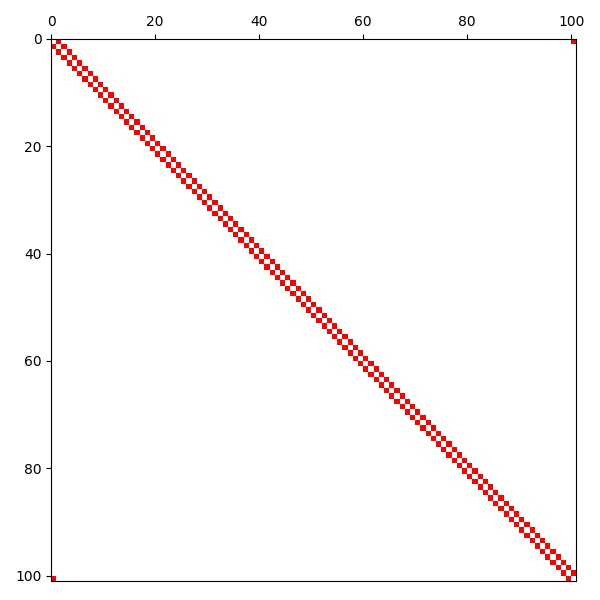
\includegraphics[width=0.5\linewidth]{./figures/results/path/graph.jpg}
\caption{Adjacency graph of the line}
\end{figure}

\begin{figure}[H]
  \centering
  \begin{subfigure}{.45\linewidth}
    \centering
    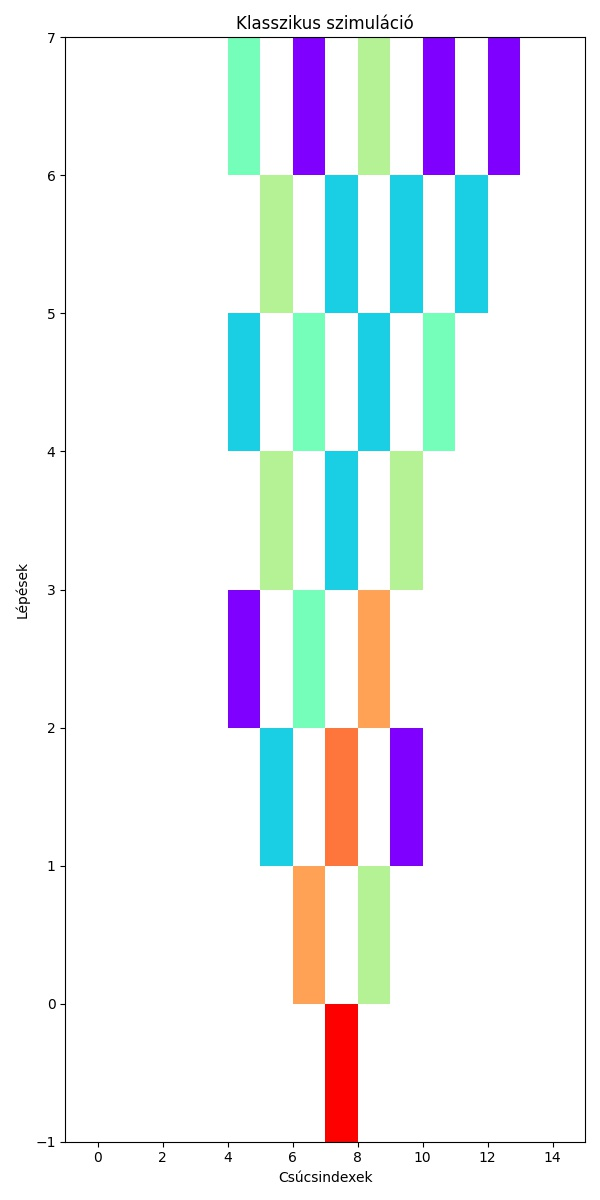
\includegraphics[width=\linewidth]{./figures/results/path/classical.jpg}
    \caption{Classical walk on the line}
  \end{subfigure}
  \begin{subfigure}{.45\linewidth}
    \centering
    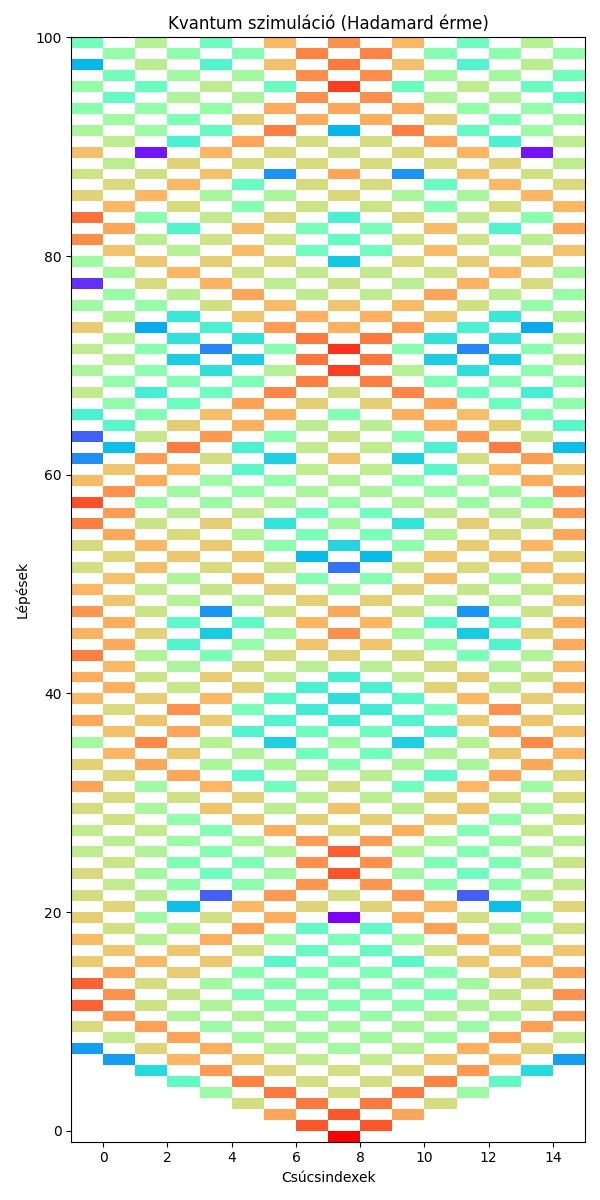
\includegraphics[width=\linewidth]{./figures/results/path/hadamard.jpg}
    \caption{Quantum walk on the line with the Hadamard coin}
  \end{subfigure}
  \caption{Walks on the line}
  \label{fig:all}
\end{figure}

\section{Walk on Grid}

\change{TODO: visszatérésről írni}

\begin{figure}[H]
\centering
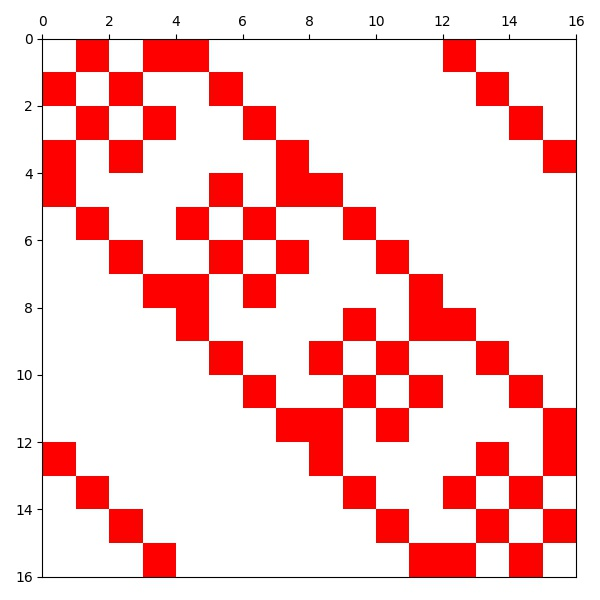
\includegraphics[width=0.5\linewidth]{./figures/results/grid/graph.jpg}
\caption{Adjacency graph of the grid}
\end{figure}

\begin{figure}[H]
  \centering
  \begin{subfigure}{.45\linewidth}
    \centering
    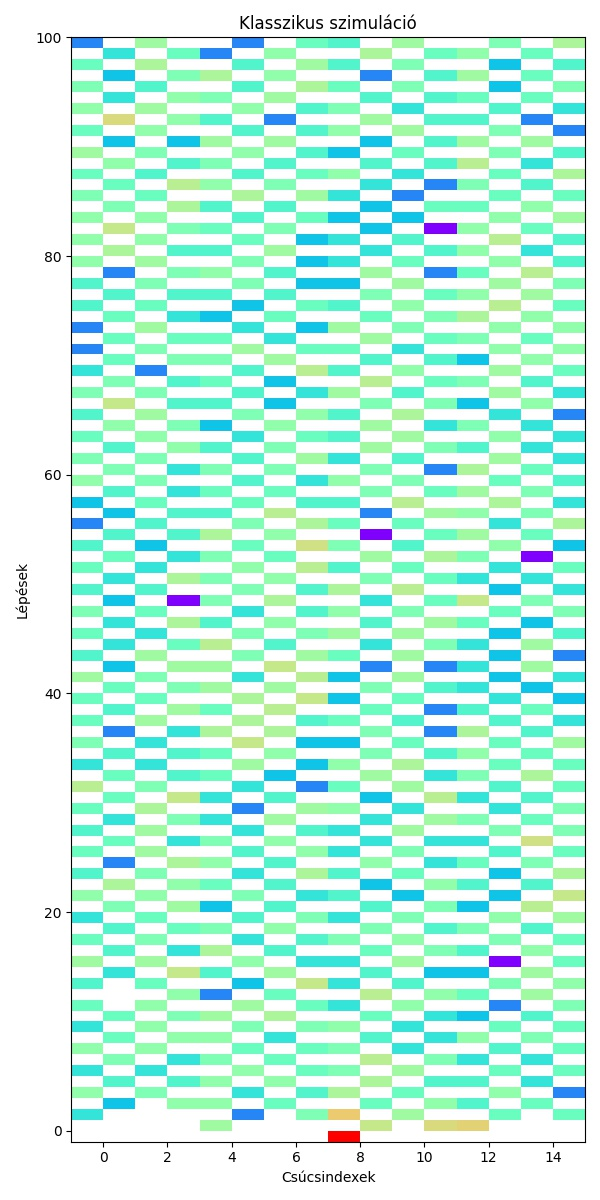
\includegraphics[width=\linewidth]{./figures/results/grid/classical.jpg}
    \caption{Classical walk on the grid}
  \end{subfigure}
  \begin{subfigure}{.45\linewidth}
    \centering
    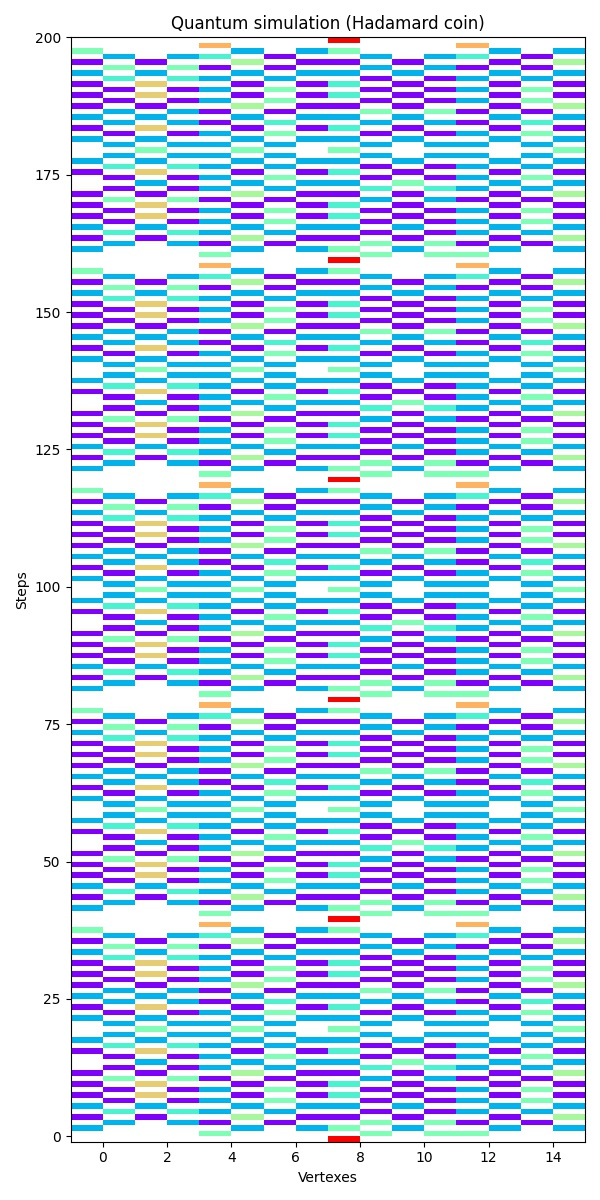
\includegraphics[width=\linewidth]{./figures/results/grid/hadamard.jpg}
    \caption{Quantum walk on the grid with the Hadamard coin}
  \end{subfigure}
  \caption{Walks on the grid}
  \label{fig:all}
\end{figure}

\begin{figure}[H]
  \centering
  \begin{subfigure}{.45\linewidth}
    \centering
    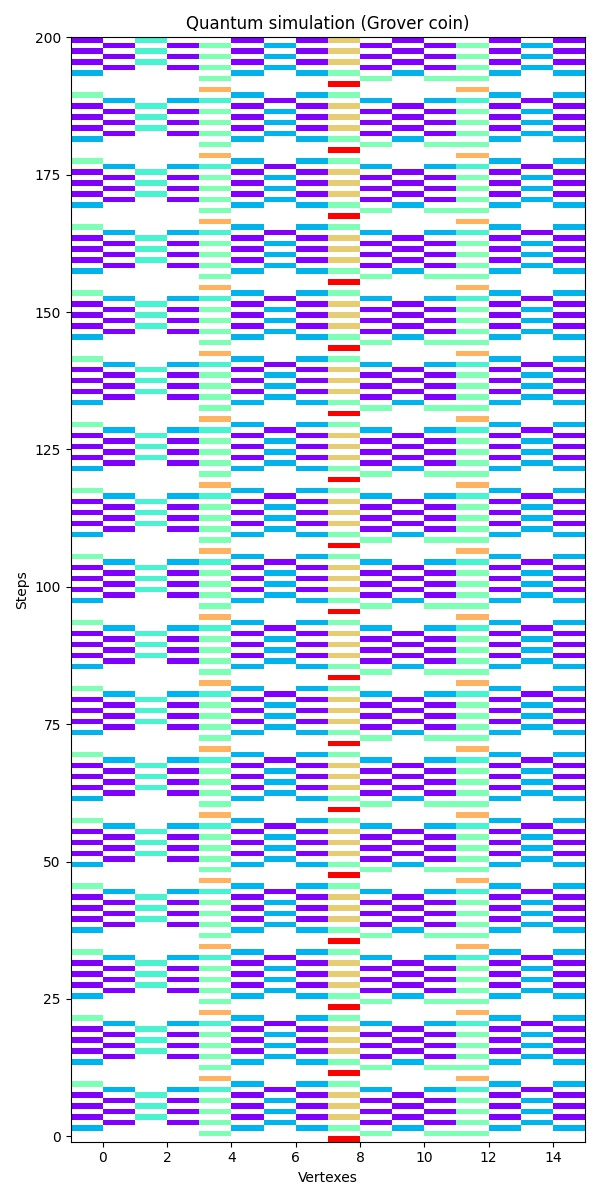
\includegraphics[width=\linewidth]{./figures/results/grid/grover.jpg}
    \caption{Quantum walk on the line with the Grover coin}
  \end{subfigure}
  \begin{subfigure}{.45\linewidth}
    \centering
    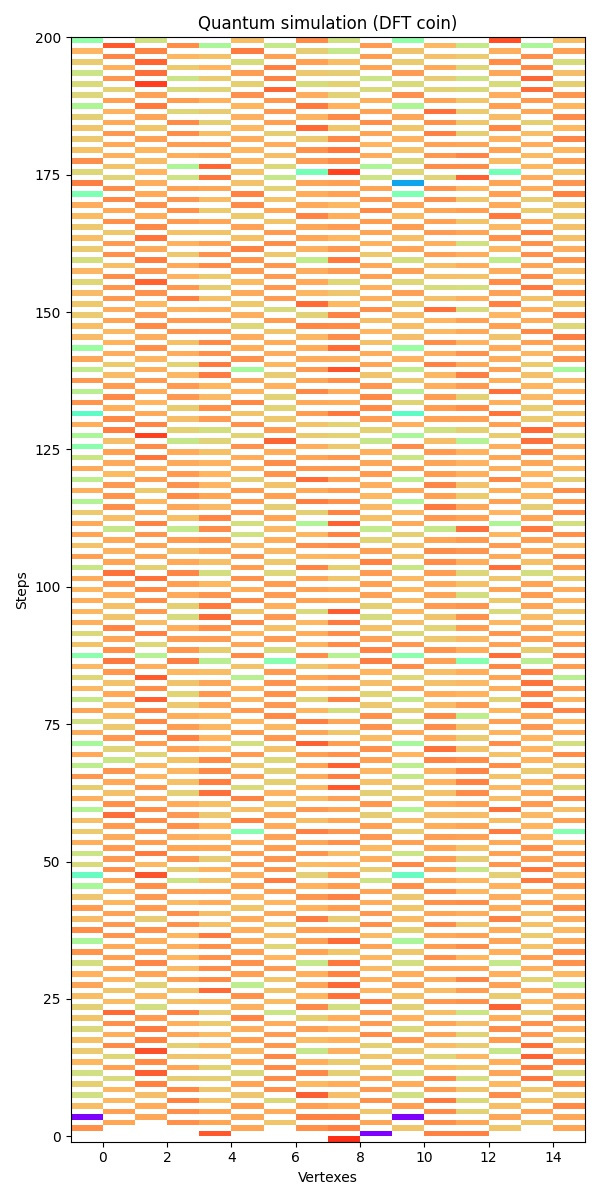
\includegraphics[width=\linewidth]{./figures/results/grid/dft.jpg}
    \caption{Quantum walk on the grid with the Fourier coin}
  \end{subfigure}
  \caption{Walks on the grid}
  \label{fig:all}
\end{figure}


\section{Walk on Hypercube}

\change{TODO: visszatérésről írni}

\begin{figure}[H]
\centering
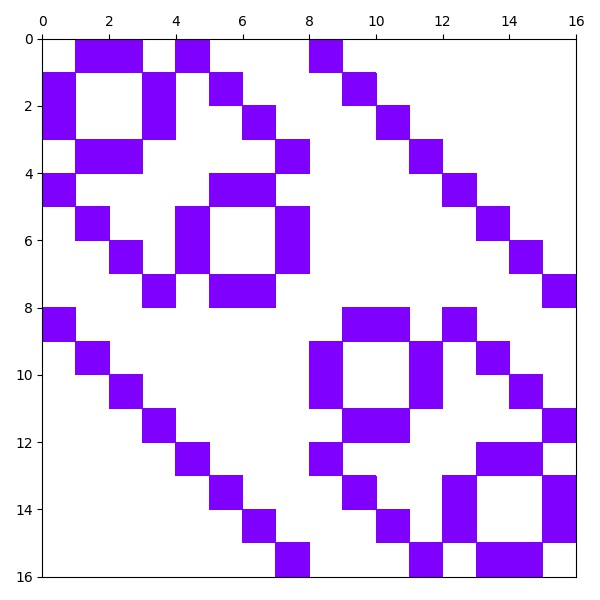
\includegraphics[width=0.5\linewidth]{./figures/results/hypercube/graph.jpg}
\caption{Adjacency graph of the hypercube}
\end{figure}

\begin{figure}[H]
  \centering
  \begin{subfigure}{.45\linewidth}
    \centering
    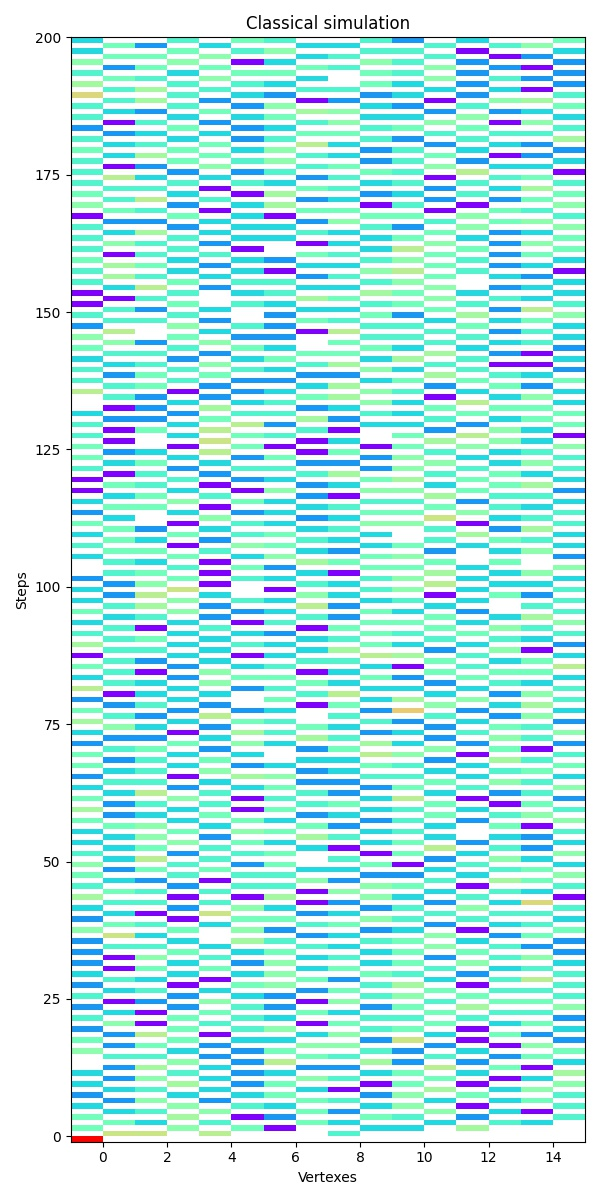
\includegraphics[width=\linewidth]{./figures/results/hypercube/classical.jpg}
    \caption{Classical walk on the hypercube}
  \end{subfigure}
  \begin{subfigure}{.45\linewidth}
    \centering
    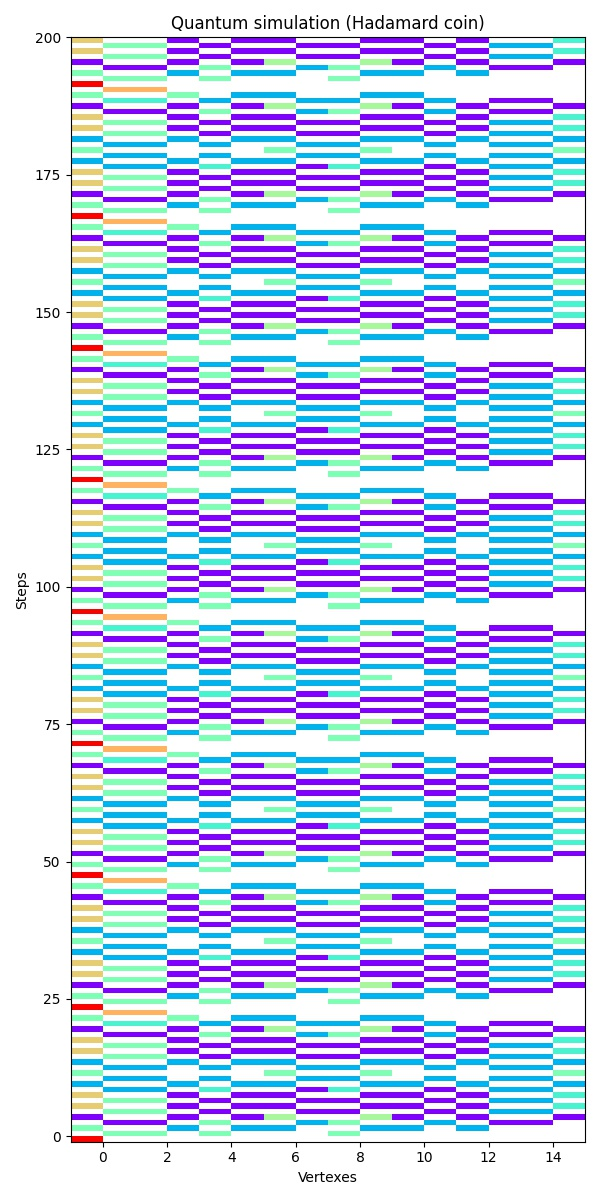
\includegraphics[width=\linewidth]{./figures/results/hypercube/hadamard.jpg}
    \caption{Quantum walk on the hypercube with the Hadamard coin}
  \end{subfigure}
  \caption{Walks on the hypercube}
  \label{fig:all}
\end{figure}

\begin{figure}[H]
  \centering
  \begin{subfigure}{.45\linewidth}
    \centering
    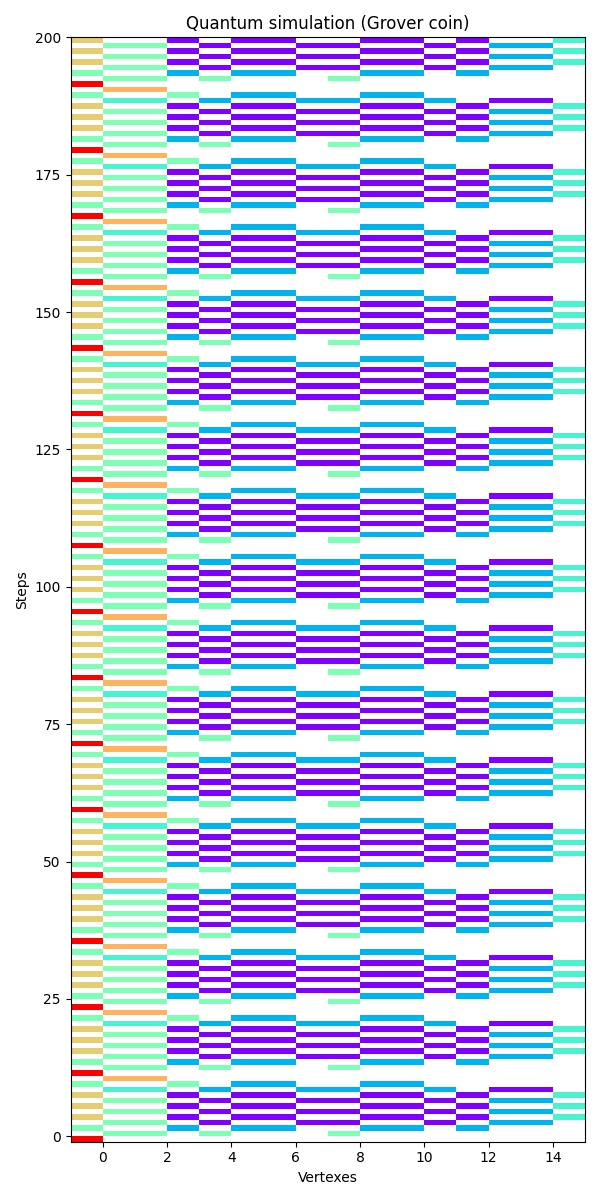
\includegraphics[width=\linewidth]{./figures/results/hypercube/grover.jpg}
    \caption{Quantum walk on the line with the Grover coin}
  \end{subfigure}
  \begin{subfigure}{.45\linewidth}
    \centering
    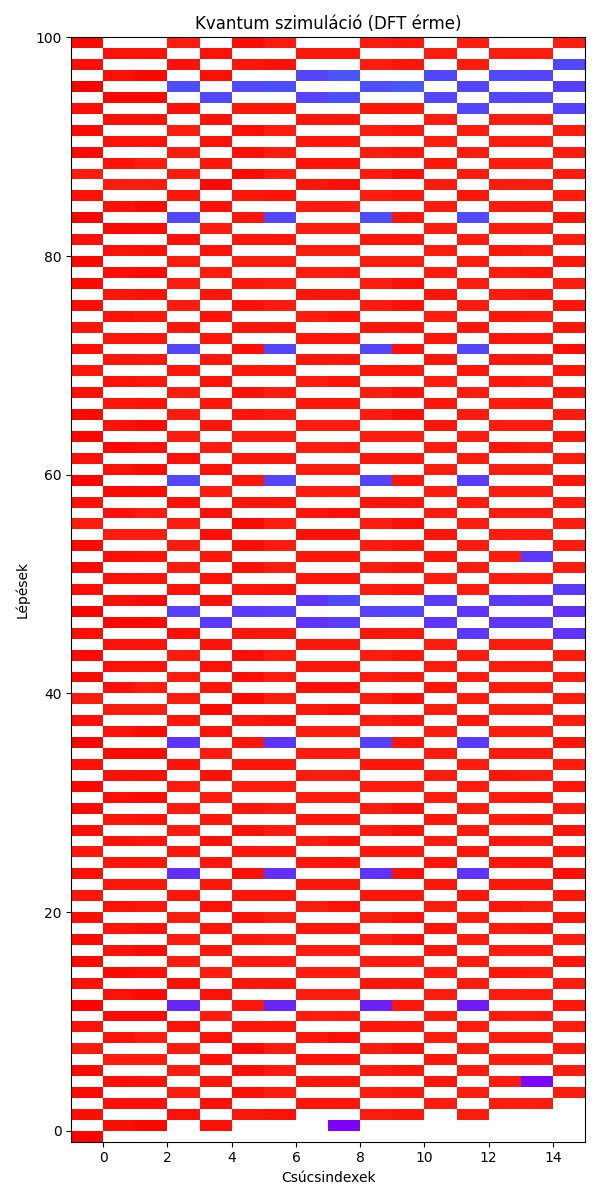
\includegraphics[width=\linewidth]{./figures/results/hypercube/dft.jpg}
    \caption{Quantum walk on the hypercube with the Fourier coin}
  \end{subfigure}
  \caption{Walks on the hypercube}
  \label{fig:all}
\end{figure}
